% Q3V2: Toroid, Opposing Dots — Physical winding diagram
% Coils wound in OPPOSITE SENSES on toroid
% Coil 1: clockwise from outside; Coil 2: counterclockwise from outside
% Does NOT show dot placements — that is Part (a) answer (P-STACK-31)
\documentclass[border=10pt]{standalone}
\usepackage{tikz}
\usepackage{amsmath}
\renewcommand{\familydefault}{\sfdefault}

\begin{document}
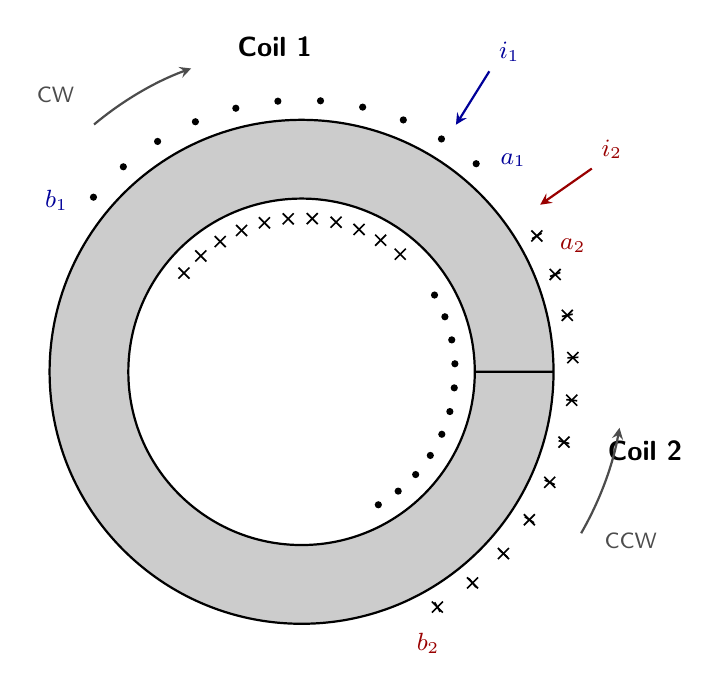
\begin{tikzpicture}[
    every node/.style={font=\sffamily},
    >=stealth,
]

% Parameters
\def\Router{3.2}
\def\Rinner{2.2}

% === Ferromagnetic core (full toroid, no gap) ===
\fill[gray!40, draw=black, line width=0.8pt]
    (0:\Router) arc (0:360:\Router)
    -- (360:\Rinner) arc (360:0:\Rinner)
    -- cycle;

% === Coil 1 (upper-left, 50-140 degrees) — clockwise from outside ===
% CW from outside → dots on outer ring, crosses on inner ring
\foreach \angle in {50,59,...,140} {
    % Outer: dot (current out of page)
    \fill ({(\Router+0.25)*cos(\angle)},{(\Router+0.25)*sin(\angle)}) circle (1.3pt);
    % Inner: cross (current into page)
    \pgfmathsetmacro{\xw}{(\Rinner-0.25)*cos(\angle)}
    \pgfmathsetmacro{\yw}{(\Rinner-0.25)*sin(\angle)}
    \draw[line width=0.6pt] ({\xw-0.07},{\yw-0.07}) -- ({\xw+0.07},{\yw+0.07});
    \draw[line width=0.6pt] ({\xw-0.07},{\yw+0.07}) -- ({\xw+0.07},{\yw-0.07});
}
% Coil 1 label
\node[above, font=\sffamily\bfseries] at ({(\Router+0.7)*cos(95)},{(\Router+0.7)*sin(95)}) {Coil 1};

% Coil 1 terminal labels (offset from current arrow to avoid overlap)
\node[font=\sffamily\small, text=blue!60!black] at ({(\Router+0.6)*cos(45)},{(\Router+0.6)*sin(45)}) {$a_1$};
\node[font=\sffamily\small, text=blue!60!black] at ({(\Router+0.6)*cos(145)},{(\Router+0.6)*sin(145)}) {$b_1$};

% Current arrow for Coil 1 (further out to separate from terminal label)
\draw[->, thick, blue!60!black]
    ({(\Router+1.3)*cos(58)},{(\Router+1.3)*sin(58)})
    -- ({(\Router+0.5)*cos(58)},{(\Router+0.5)*sin(58)});
\node[above right, font=\sffamily\small, text=blue!60!black]
    at ({(\Router+1.3)*cos(58)},{(\Router+1.3)*sin(58)}) {$i_1$};

% === Coil 2 (lower-right, -60 to 30 degrees) — OPPOSITE sense ===
% CCW from outside → crosses on outer ring, dots on inner ring (reversed!)
\foreach \angle in {-60,-51,...,30} {
    % Outer: CROSS (reversed from Coil 1)
    \draw[line width=0.6pt]
        ({(\Router+0.18)*cos(\angle)},{(\Router+0.18)*sin(\angle)})
        -- ({(\Router+0.32)*cos(\angle)},{(\Router+0.32)*sin(\angle)});
    \pgfmathsetmacro{\xo1}{(\Router+0.18)*cos(\angle)+0.07*sin(\angle)}
    \pgfmathsetmacro{\yo1}{(\Router+0.18)*sin(\angle)-0.07*cos(\angle)}
    \pgfmathsetmacro{\xo2}{(\Router+0.32)*cos(\angle)-0.07*sin(\angle)}
    \pgfmathsetmacro{\yo2}{(\Router+0.32)*sin(\angle)+0.07*cos(\angle)}
    % Simplified cross marks
    \pgfmathsetmacro{\cx}{(\Router+0.25)*cos(\angle)}
    \pgfmathsetmacro{\cy}{(\Router+0.25)*sin(\angle)}
    \draw[line width=0.6pt] ({\cx-0.07},{\cy-0.07}) -- ({\cx+0.07},{\cy+0.07});
    \draw[line width=0.6pt] ({\cx-0.07},{\cy+0.07}) -- ({\cx+0.07},{\cy-0.07});
    % Inner: DOT (reversed from Coil 1)
    \fill ({(\Rinner-0.25)*cos(\angle)},{(\Rinner-0.25)*sin(\angle)}) circle (1.3pt);
}
% Coil 2 label
\node[right, font=\sffamily\bfseries] at ({(\Router+0.7)*cos(-15)},{(\Router+0.7)*sin(-15)}) {Coil 2};

% Coil 2 terminal labels (offset from current arrow)
\node[font=\sffamily\small, text=red!60!black] at ({(\Router+0.6)*cos(25)},{(\Router+0.6)*sin(25)}) {$a_2$};
\node[font=\sffamily\small, text=red!60!black] at ({(\Router+0.6)*cos(-65)},{(\Router+0.6)*sin(-65)}) {$b_2$};

% Current arrow for Coil 2 (further out)
\draw[->, thick, red!60!black]
    ({(\Router+1.3)*cos(35)},{(\Router+1.3)*sin(35)})
    -- ({(\Router+0.5)*cos(35)},{(\Router+0.5)*sin(35)});
\node[above right, font=\sffamily\small, text=red!60!black]
    at ({(\Router+1.3)*cos(35)},{(\Router+1.3)*sin(35)}) {$i_2$};

% === Winding sense annotations ===
\draw[->, thick, gray!60!black]
    ({(\Router+0.9)*cos(130)},{(\Router+0.9)*sin(130)})
    arc[start angle=130, end angle=110, radius=\Router+0.9];
\node[above left, font=\sffamily\footnotesize, gray!60!black]
    at ({(\Router+1.1)*cos(130)},{(\Router+1.1)*sin(130)}) {CW};

\draw[<-, thick, gray!60!black]
    ({(\Router+0.9)*cos(-10)},{(\Router+0.9)*sin(-10)})
    arc[start angle=-10, end angle=-30, radius=\Router+0.9];
\node[right, font=\sffamily\footnotesize, gray!60!black]
    at ({(\Router+1.1)*cos(-30)},{(\Router+1.1)*sin(-30)}) {CCW};

\end{tikzpicture}
\end{document}
